%TCIDATA{LaTeXparent=0,0,relatorio.tex}
\chapter{Resultados\label{chap:Resultados}}

% Resumo opcional. Comentar se não usar.
\resumodocapitulo{Este capítulo apresenta os procedimentos experimentais realizados e seus resultados.}


\section{Câmera}
\subsection{Calibração}

%TODO Pegar printscreens do programa que roda na câmera
A câmera permite fazer medidas de distâncias em pixels. De forma a se converter essa distância para milímetros, uma barra de alumínio com marcas e tamanho conhecido é utilizada. É importante primeiro calibrar o sistema, para se saber se há deformação de pixels significante ao longo da distância de interesse. No PresencePlus P4 GEO 1.3, um programa com imagem de referência é feito, conforme Figura .... A barra de alumínio atualmente utilizada tem comprimento total de $532$mm. Algumas marcas foram feitas e a Tabela \ref{relacoesmmpx} apresenta os resultados para cada seção. A distância entre duas marcas é de 10cm.
%TODO - obter imagem de referência e referenciar no parágrafo acima

\begin{table}[!ht]
\centering
\caption{Relações mm/px para diferentes seções da barra de alumínio \label{relacoesmmpx}}
	\begin{tabular}{|c|c|c|c|}
	\hline
		Seção 1 & Seção 2 & Distância (px) & mm/px\\ \hline
		P0 & P10 & 160 & 0.625\\ \hline
		P10 & P20 & 173 & 0.578\\ \hline
		P20 & P30 & 176 & 0.568\\ \hline
		P30 & P40 & 173 & 0.578\\ \hline
		P40 & P50 & 163 & 0.613\\ \hline
		P0 & PEND & 893 & 0.596\\ \hline
	\end{tabular}
\end{table}

O maior desvio da quantidade de milímetros por pixels das seções em relação à da barra inteira é de aproximadamente 4.93\%. Há algumas imprecisões na maneira como os traços foram desenhados e é possível que o erro seja menor.

\subsection{Programação}

\section{Calibração do Servomotor}

\begin{table}[!ht]
\centering
\caption{Dados de calibração do servomotor, média obtida é de 71.32 mm/unidade}
\begin{tabular}{|c|c|c|c|c|c|}
\hline
	$x_0$ - [mm] & $x_f$ - [mm] & $\Delta t$ - [seg] & Velocidade - [mm/s] & Velocidade - [u/s] & mm/u\\ \hline
2 &	71.8  &	2   &	0.5 &	34.9   & 	69.8\\ \hline
6 & 76.1  &	2   &	0.5 &	35.05  &	70.1\\ \hline
6 &	188	  &  5   &	0.5	&   36.4   &	72.8\\ \hline
6 &	185   &	2.5 &	1	& 	71.6   &	71.6\\ \hline
6 &	77    &	10  &	0.1	&   7.1    &	71\\ \hline
6 &	296.5 &	20	&   0.2 & 	14.525 &	72.625\\ \hline\end{tabular}
\end{table}

\section{Malha aberta}

O planejamento de trajetória em malha aberta e malha fechada para o \textit{riser} que está sendo utilizado neste trabalho foi desenvolvido por Fabrício et al \cite{fabricioIFAC}. Um programa em MATLAB foi escrito e gerou trajetórias de excursão pré-definida. Rédytton \cite{redytton} testou o sistema para uma excursão de cerca de 1m, que é maior que o tamanho do barbante (82cm) conforme apresentado na Tabela ....

\subsection{Excursão de 30cm}
\begin{figure}[!htb]
    \centering
    \begin{minipage}{.45\textwidth}
        \centering
        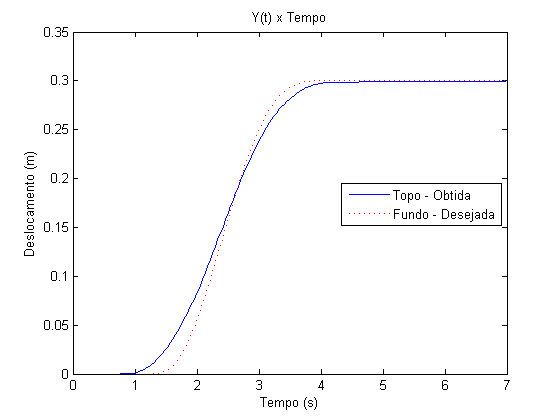
\includegraphics[width=1\linewidth]{figs/resultados/malha_aberta_1/DeslocamentoT1}
        \caption{Referência de Posição para Excursão de 30cm}
        \label{DeslocamentoT1}
    \end{minipage}%
    \hspace{0.1cm}
    \begin{minipage}{0.45\textwidth}
        \centering
        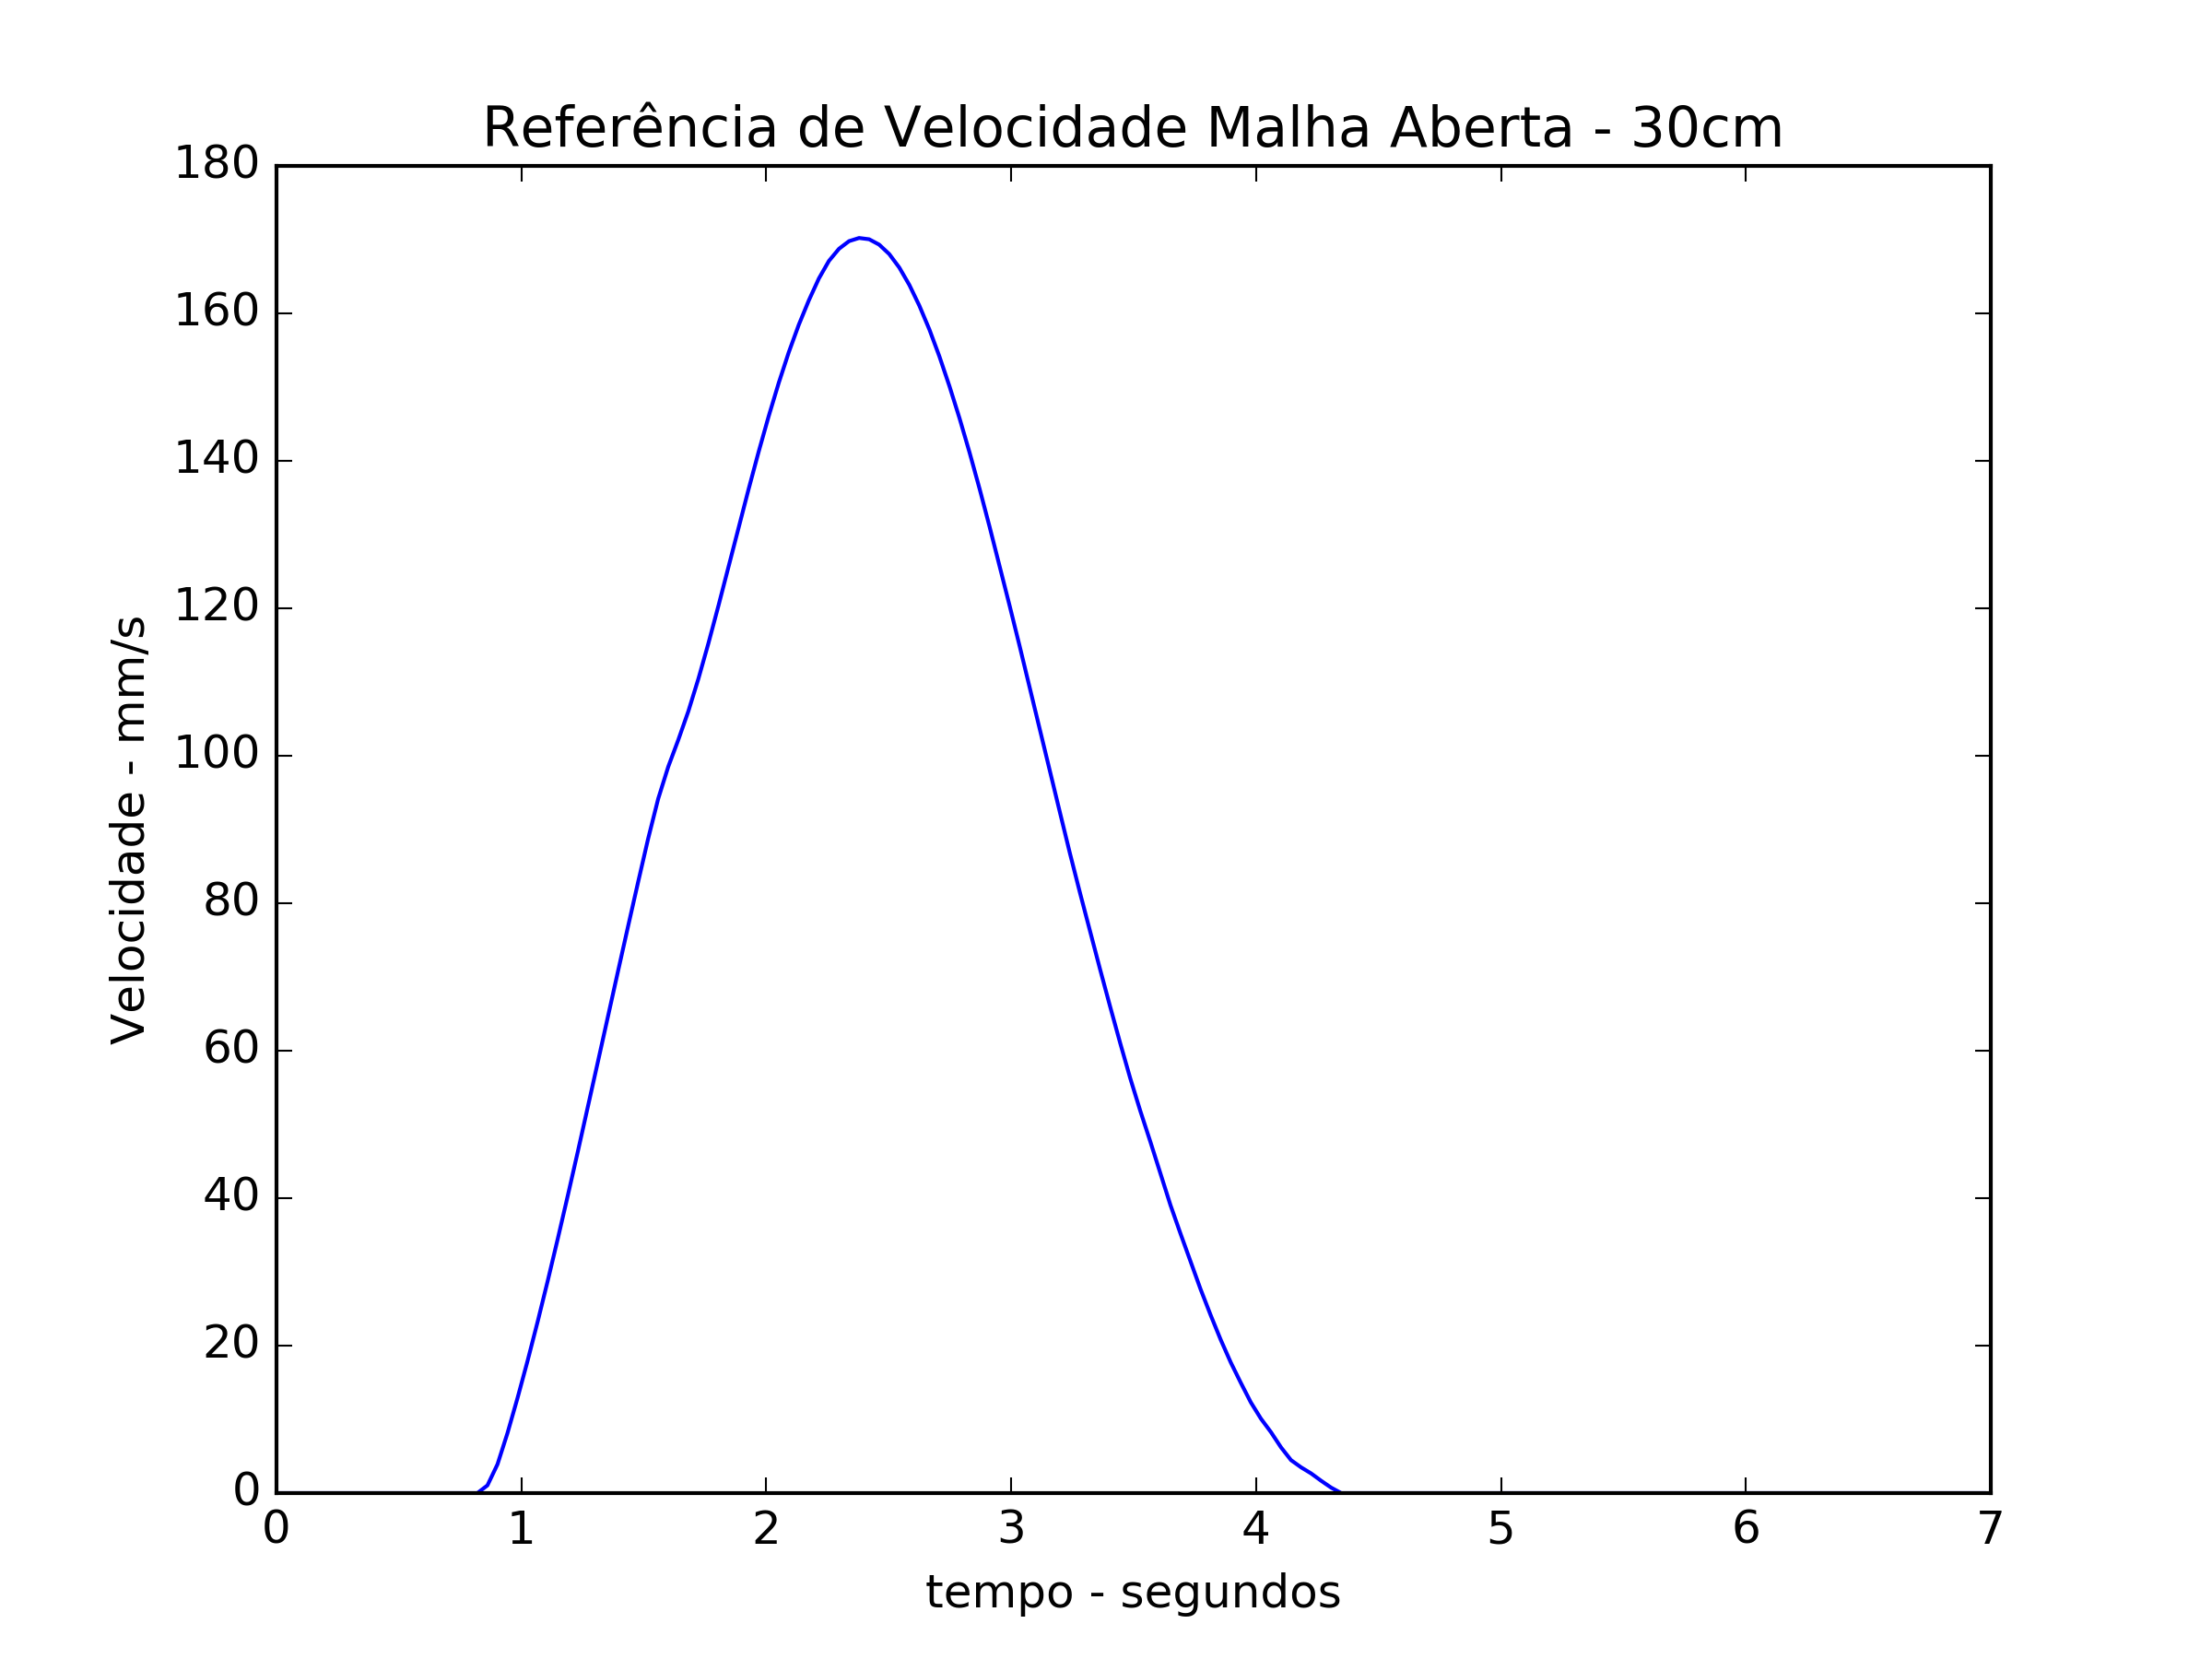
\includegraphics[width=1\linewidth]{figs/resultados/malha_aberta_1/VelocidadeT1}
        \caption{Referência de Velocidade para Excursão de 30cm}
        \label{VelocidadeT1}
    \end{minipage}
\end{figure}

\begin{figure}[!htb]
    \centering
    \begin{minipage}{.45\textwidth}
        \centering
        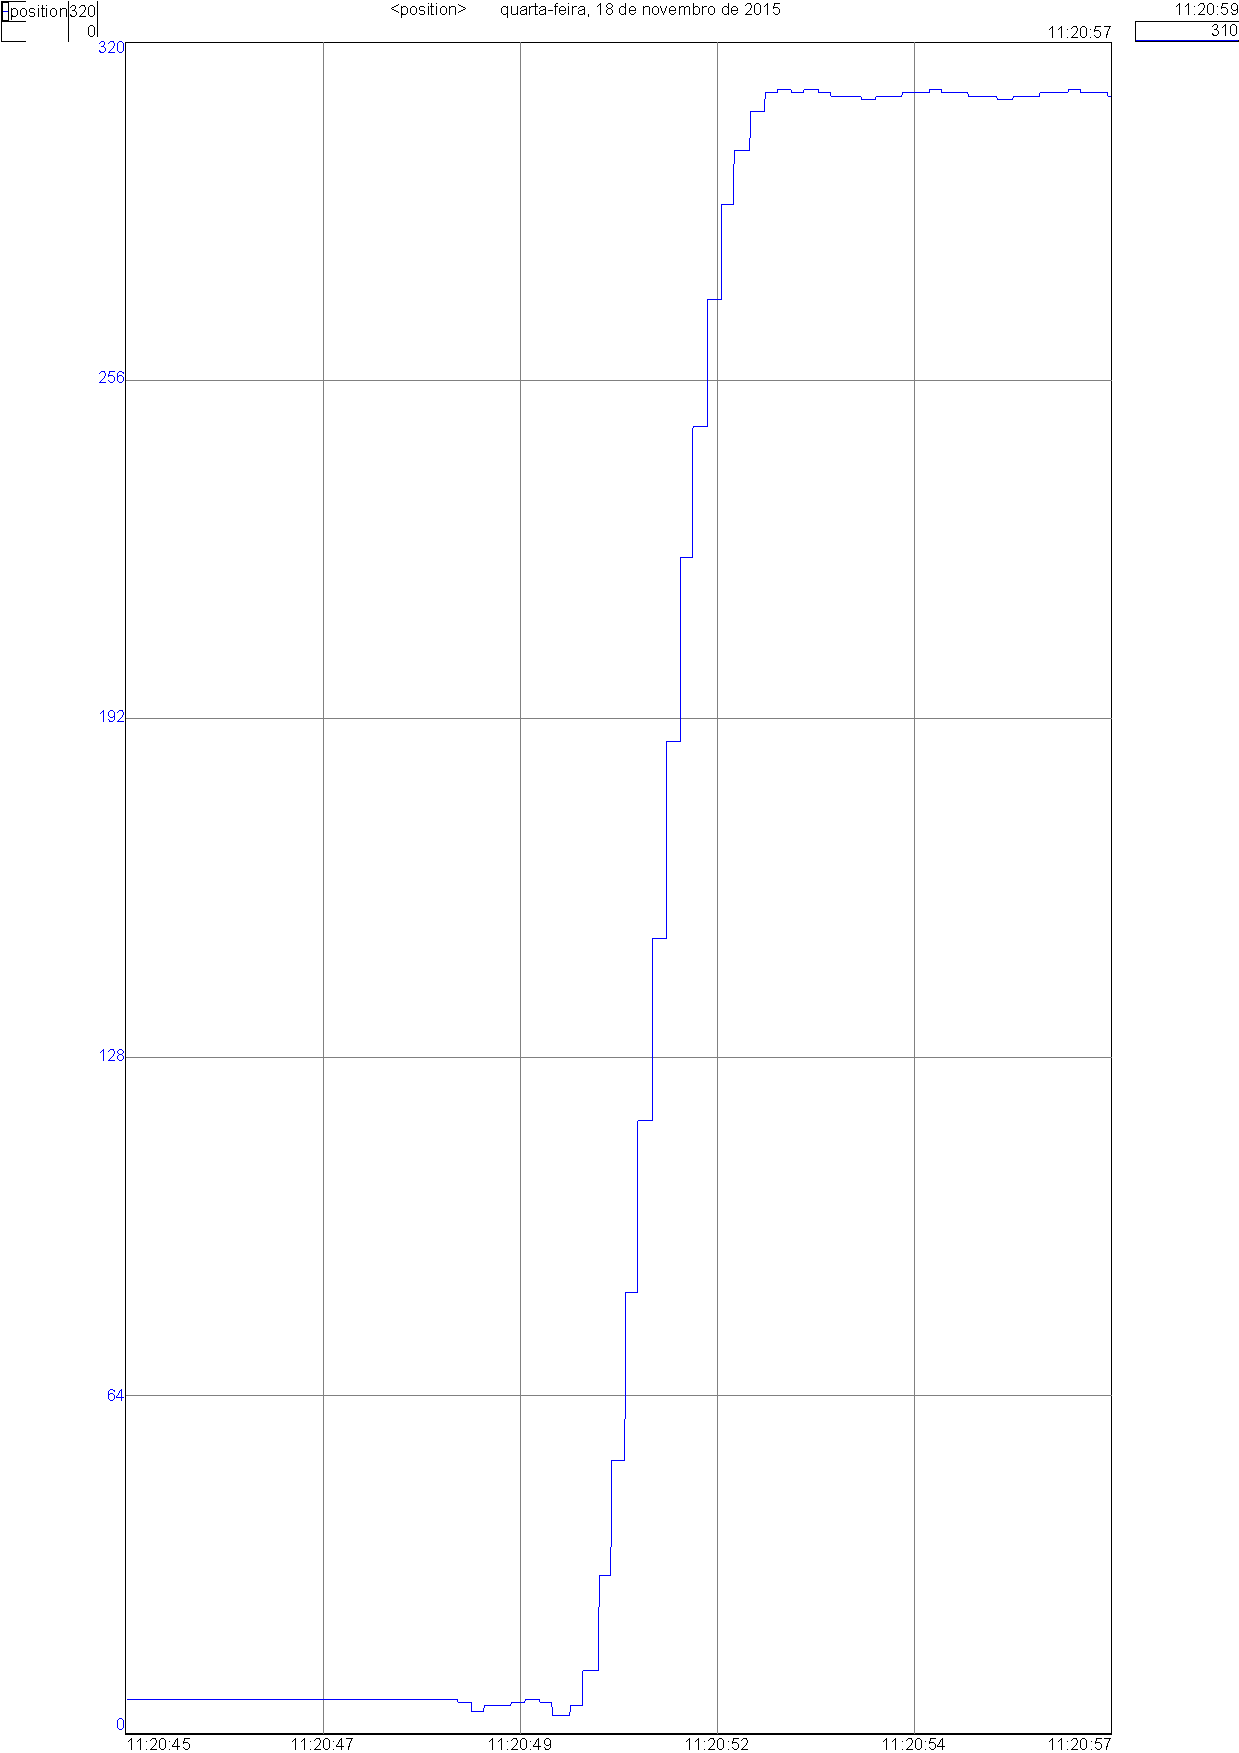
\includegraphics[width=1\linewidth,height=6cm]{figs/resultados/malha_aberta_1/trajetoriaObtidaModelada.pdf}
        \caption{Resultado com Velocidade Modelada para Excursão de 30cm}
        \label{trajetoriaObtidaModelada}
    \end{minipage}%
    \hspace{0.1cm}
    \begin{minipage}{0.45\textwidth}
        \centering
        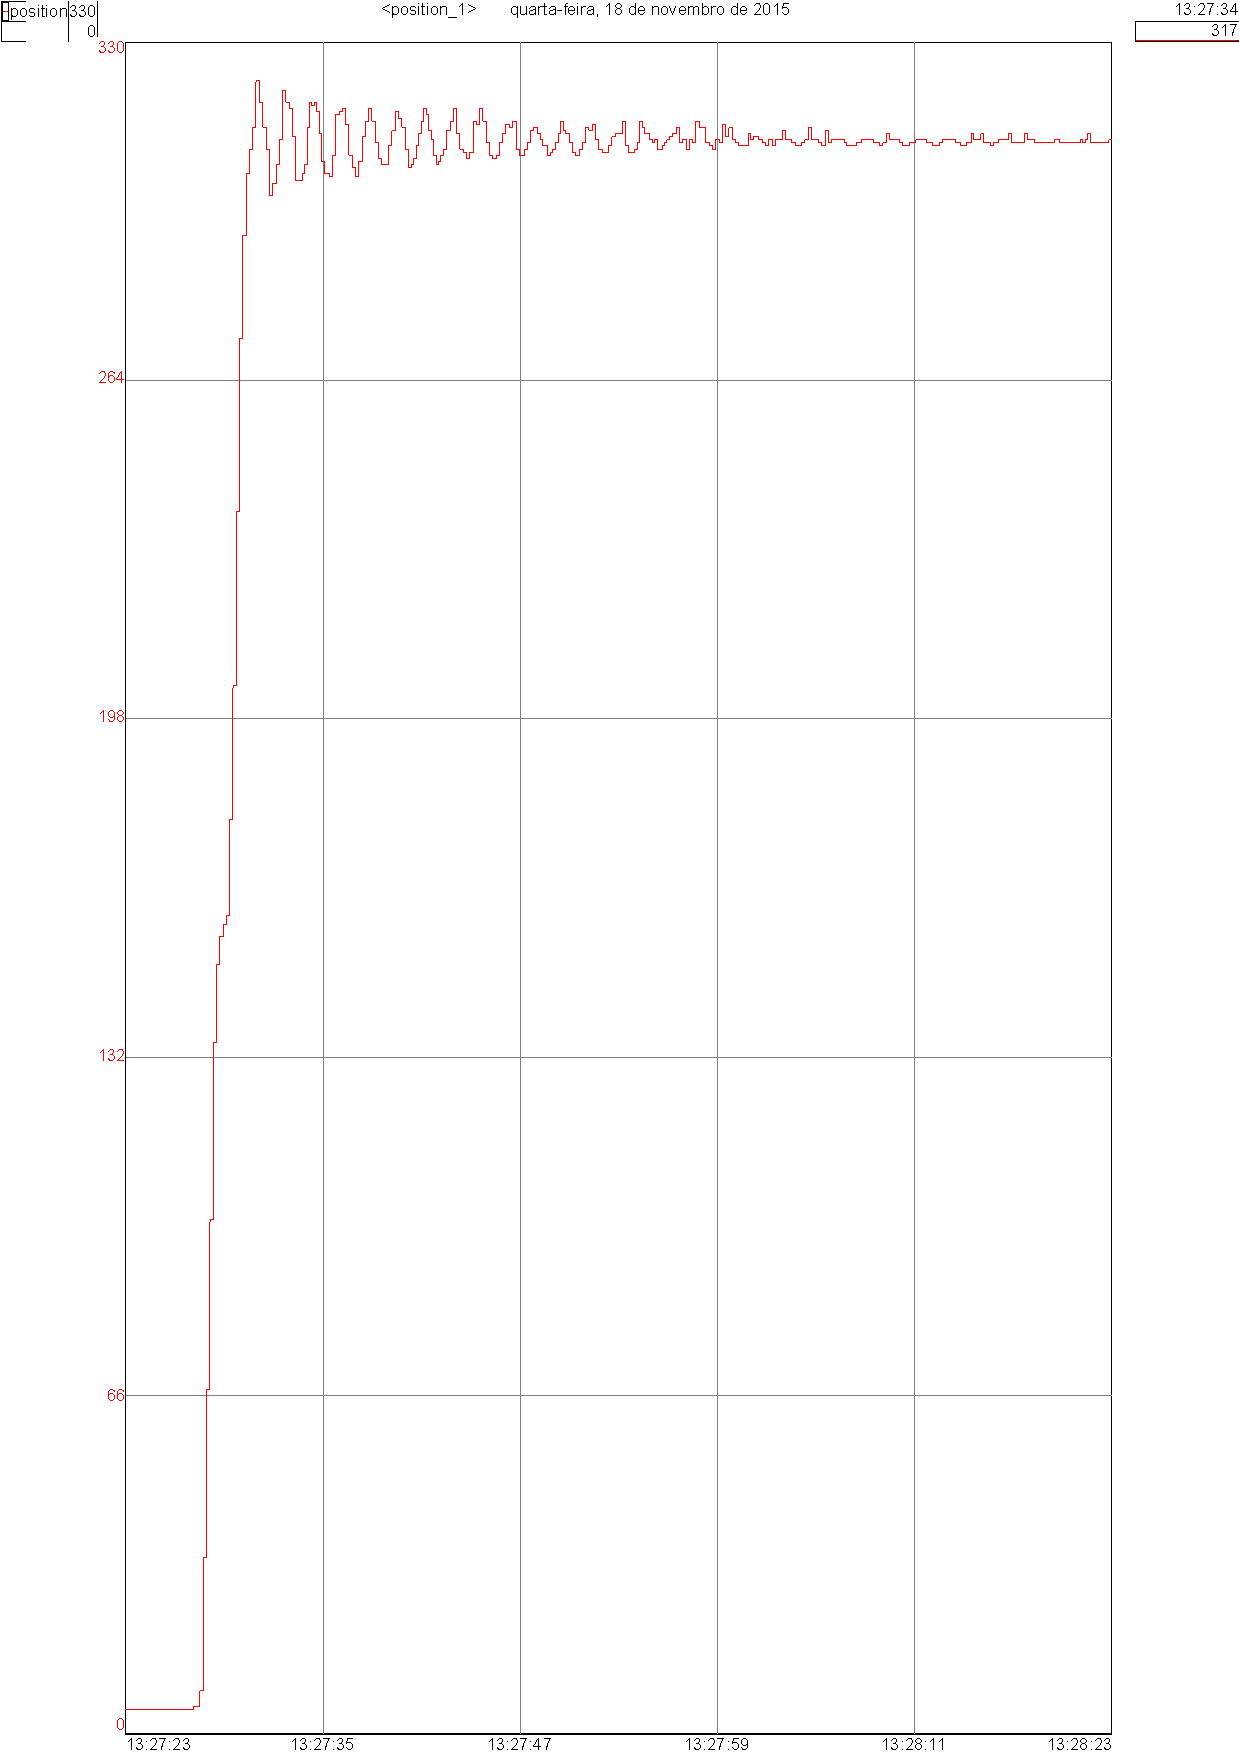
\includegraphics[width=1\linewidth,height=6cm]{figs/resultados/malha_aberta_1/trajetoriaObtidaVConstante.pdf}
        \caption{Resultado com Velocidade Constante para Excursão de 30cm}
        \label{trajetoriaObtidaVConstante}
    \end{minipage}
\end{figure}

\subsection{Excursão de 20cm}
\begin{figure}[!htb]
    \centering
    \begin{minipage}{.45\textwidth}
        \centering
        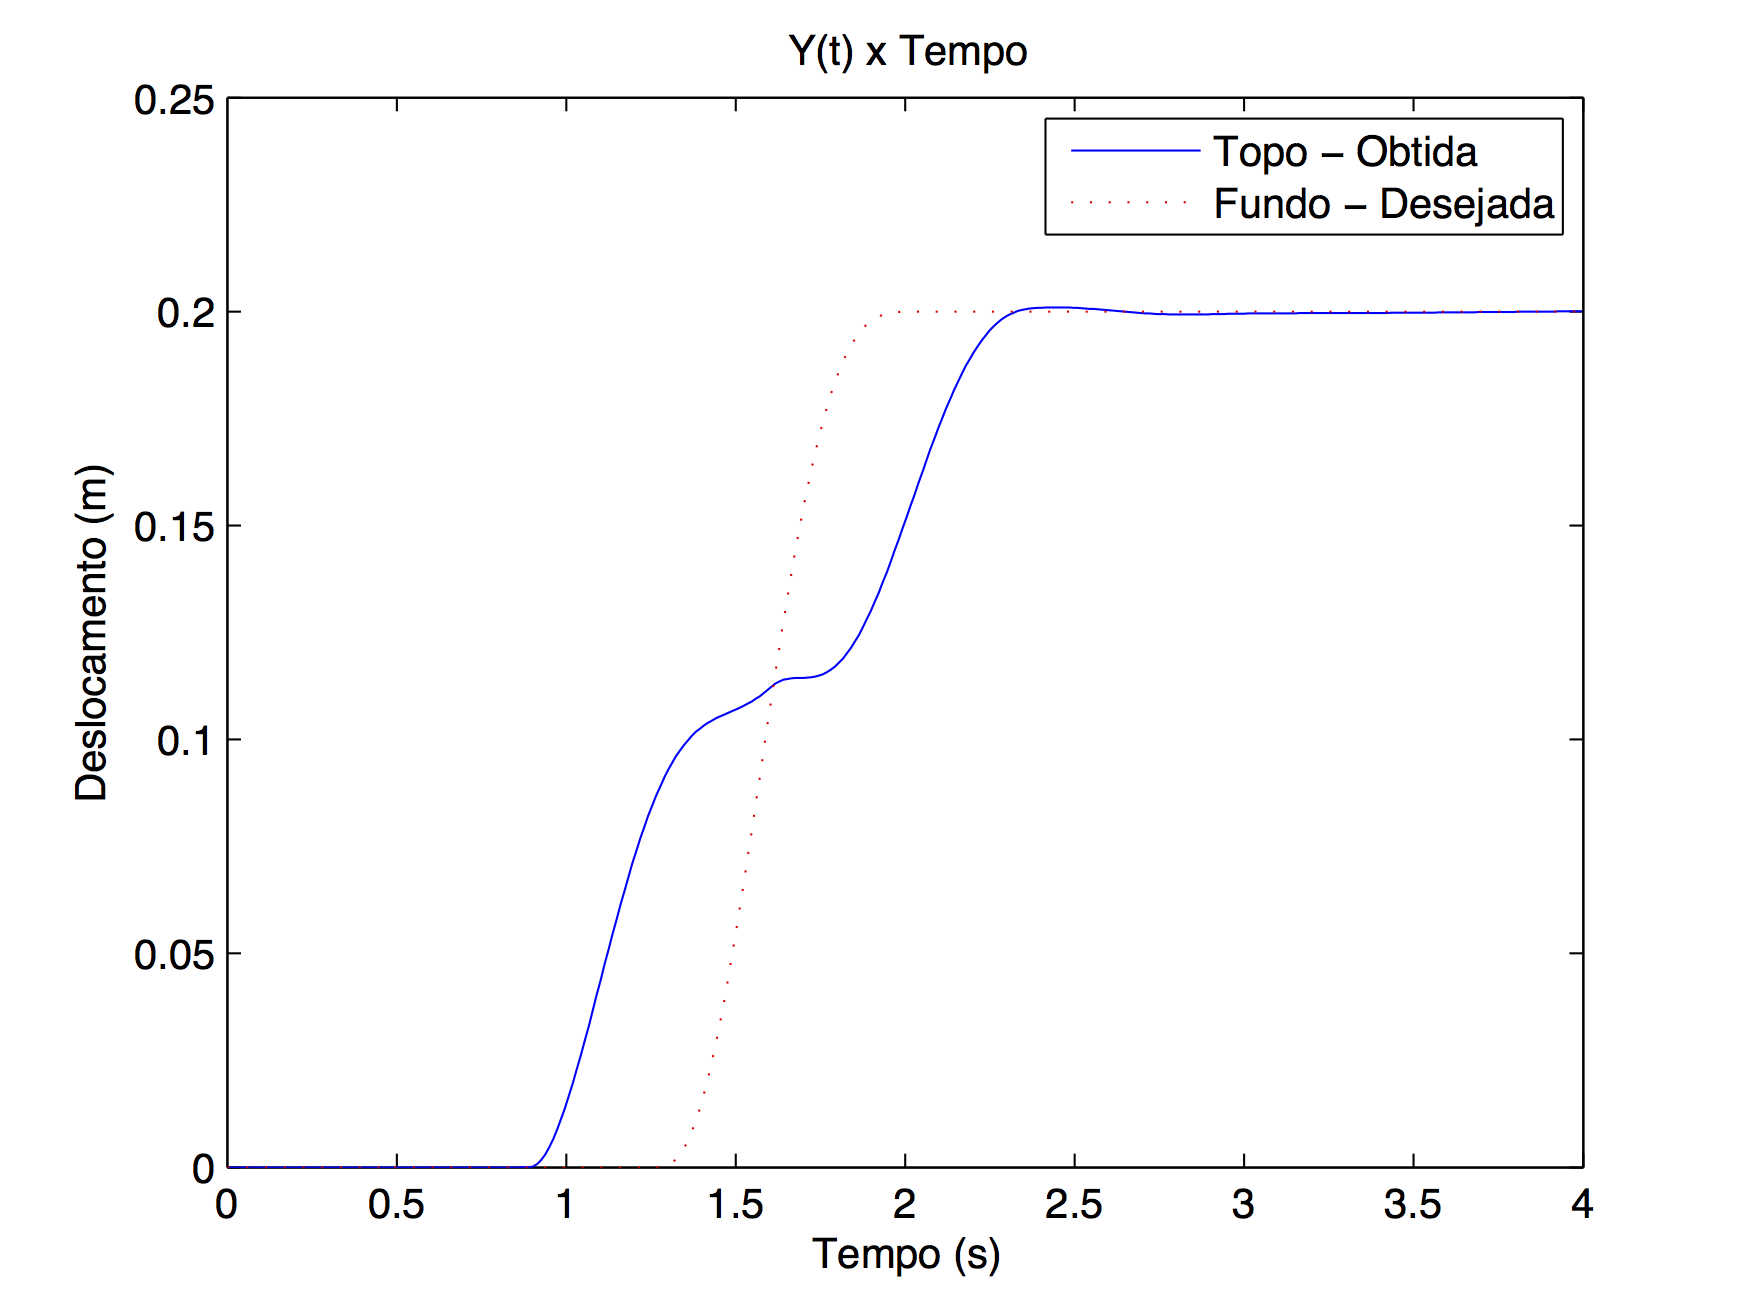
\includegraphics[width=1\linewidth]{figs/resultados/malha_aberta_2/DeslocamentoT2}
        \caption{Referência de Posição para Excursão de 20cm}
        \label{DeslocamentoT2}
    \end{minipage}%
    \hspace{0.1cm}
    \begin{minipage}{0.45\textwidth}
        \centering
        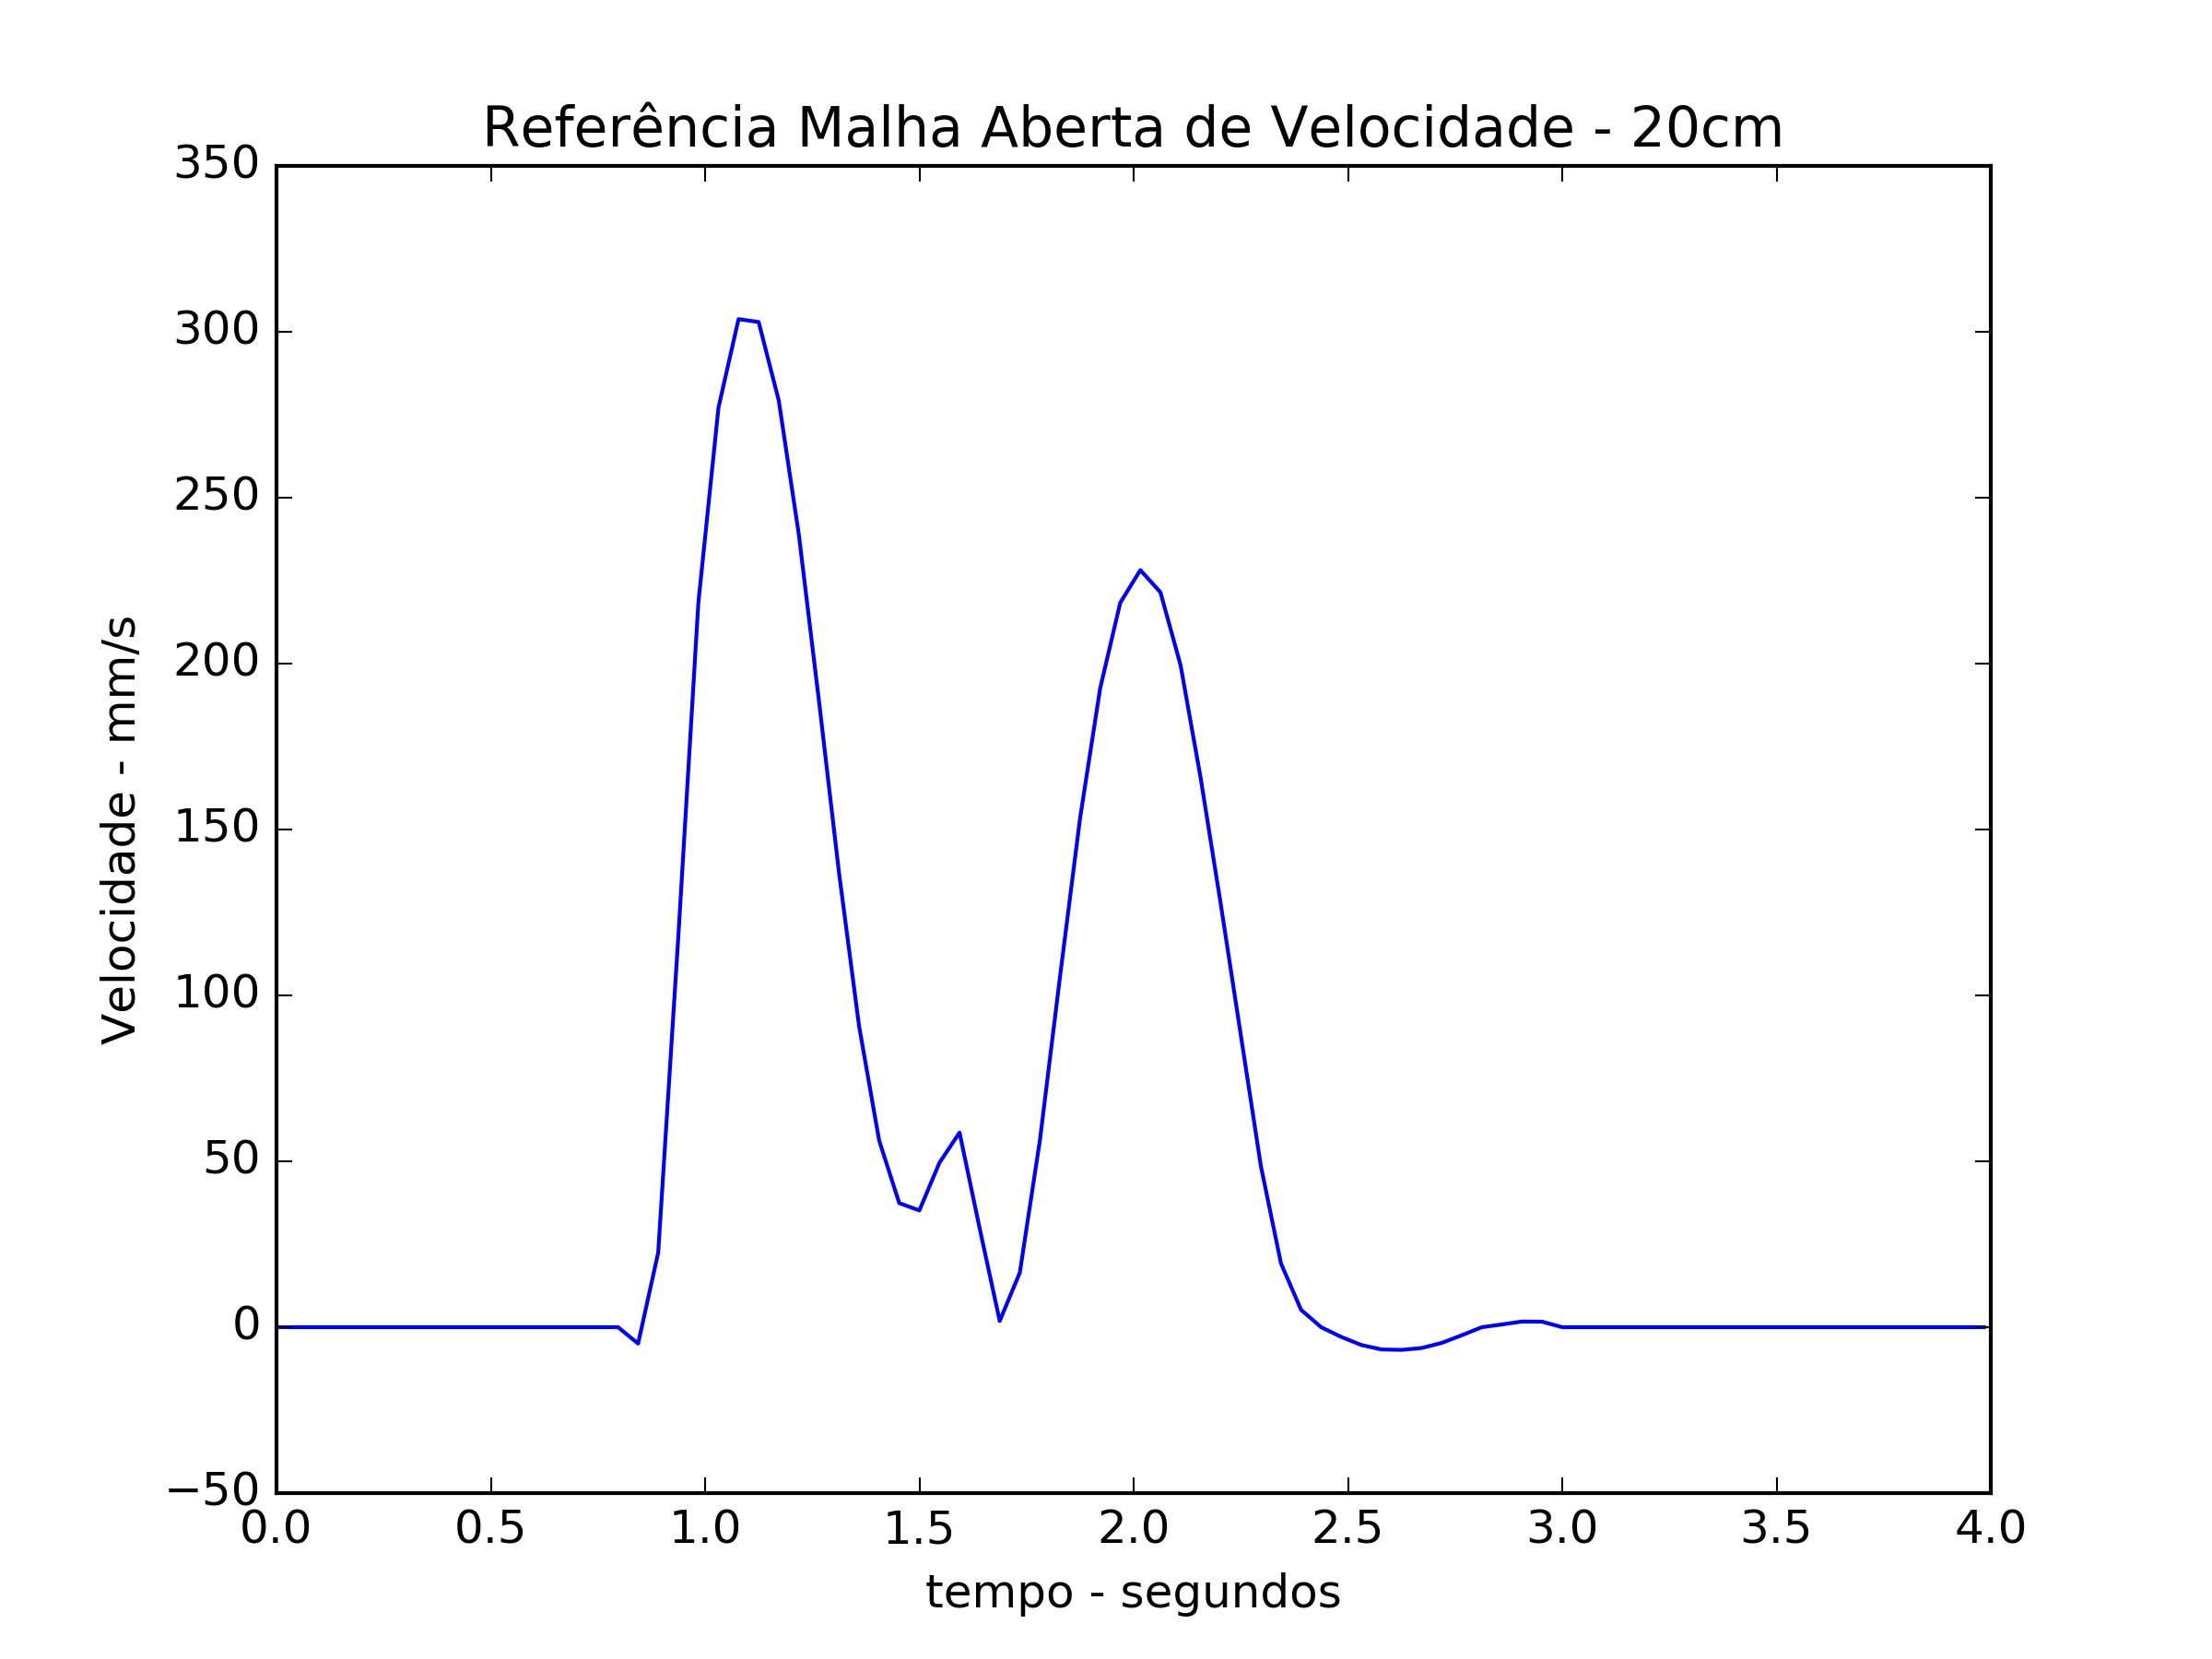
\includegraphics[width=1\linewidth]{figs/resultados/malha_aberta_2/VelocidadeT2}
        \caption{Referência de Velocidade para Excursão de 20cm}
        \label{VelocidadeT2}
    \end{minipage}
\end{figure}

\begin{figure}[!htb]
    \centering
    \begin{minipage}{.45\textwidth}
        \centering
        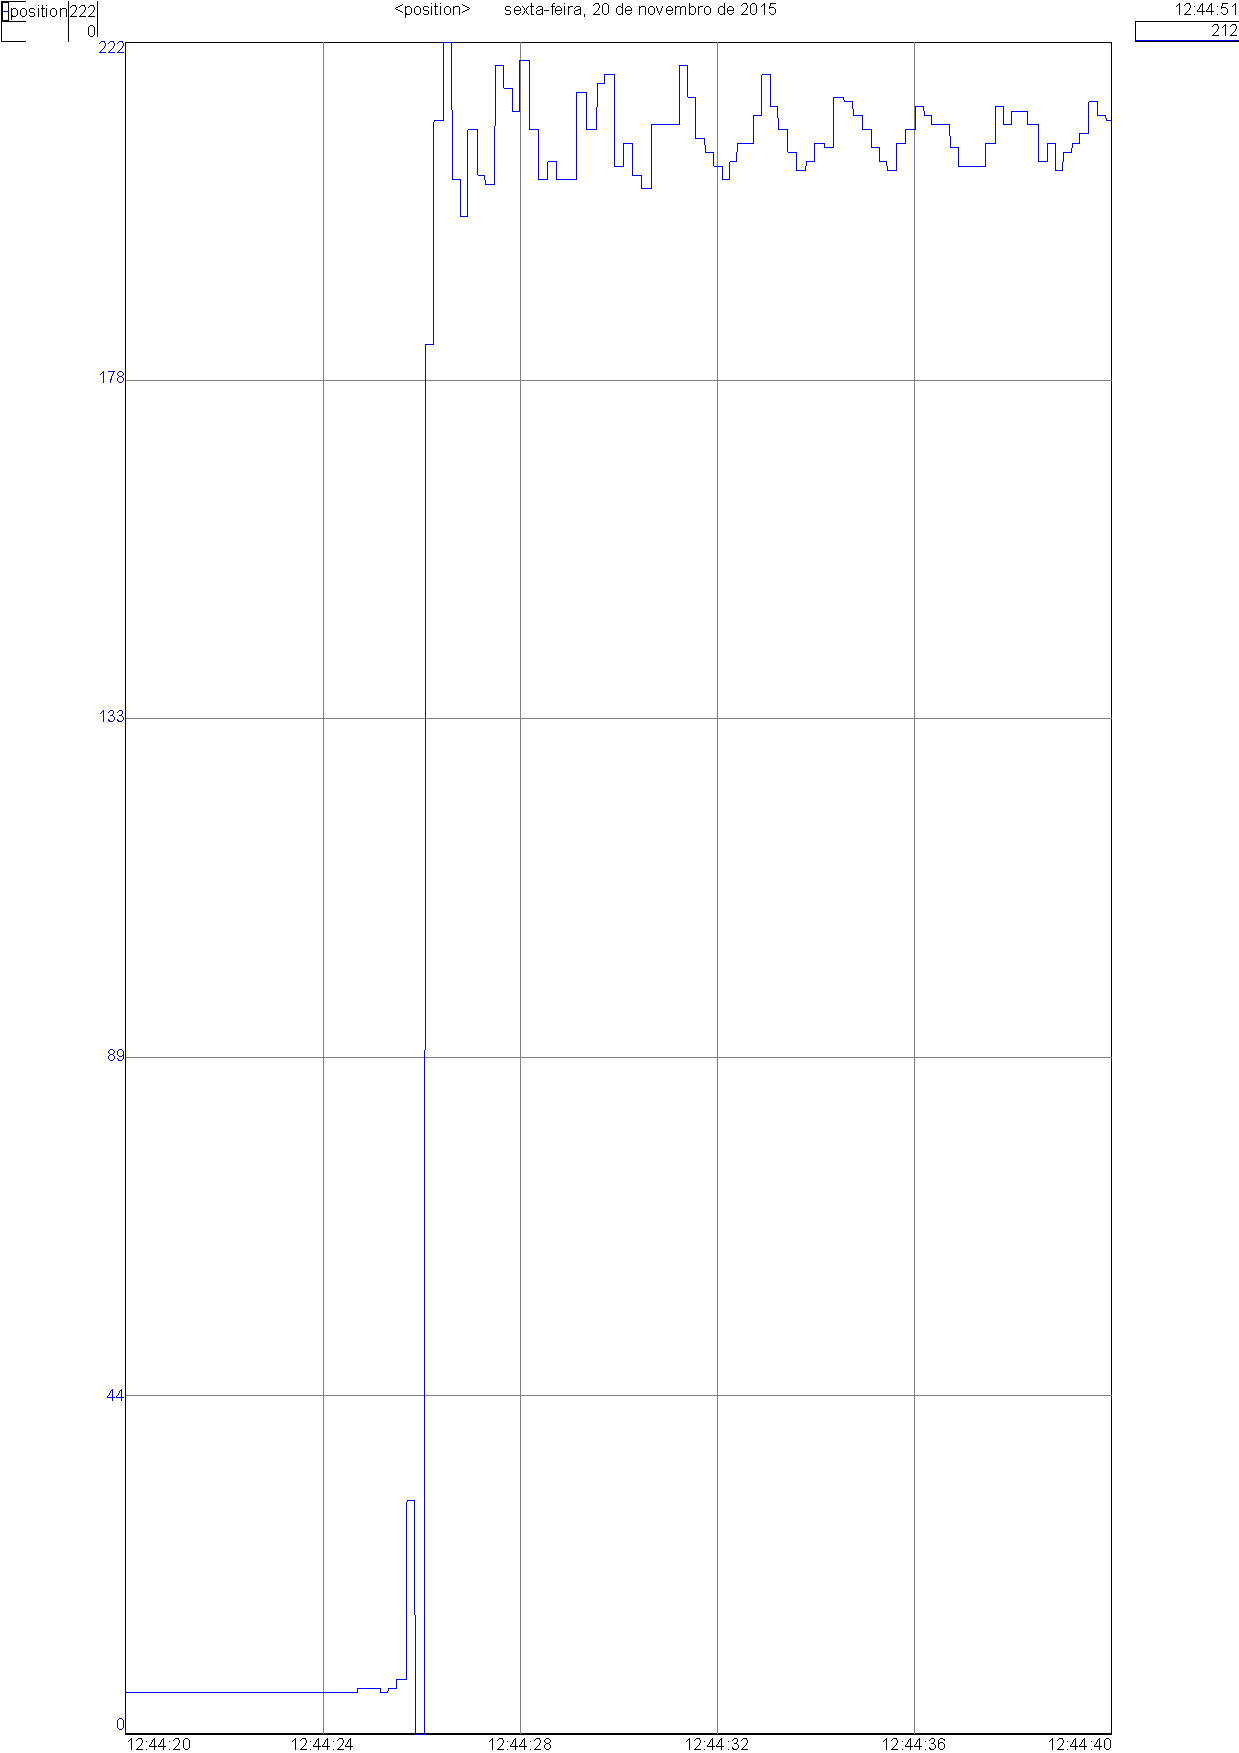
\includegraphics[width=1\linewidth,height=6cm]{figs/resultados/malha_aberta_2/percurso20cmBom.pdf}
        \caption{Resultado com Velocidade Modelada para Excursão de 20cm}
        \label{percurso20cmBom}
    \end{minipage}%
    \hspace{0.1cm}
    \begin{minipage}{0.45\textwidth}
        \centering
        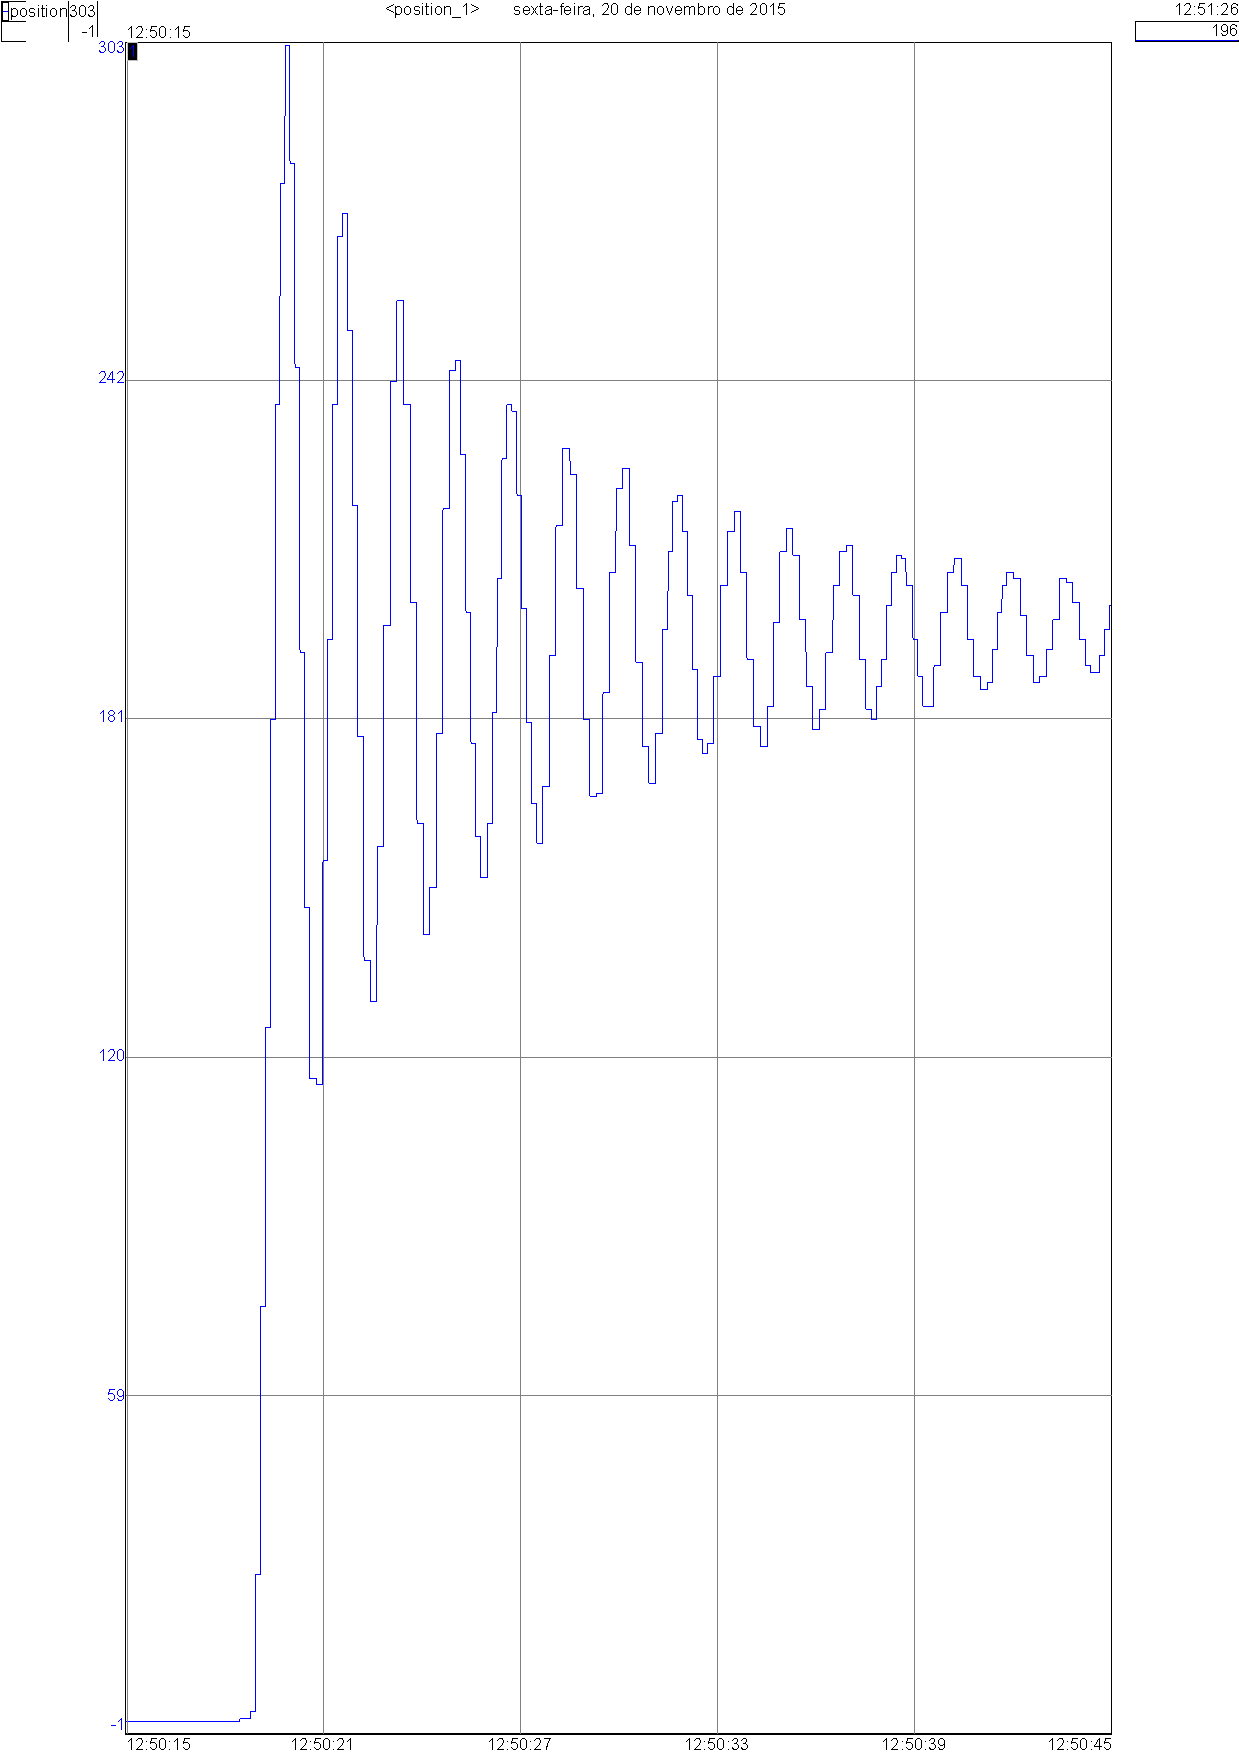
\includegraphics[width=1\linewidth,height=6cm]{figs/resultados/malha_aberta_2/percurso20cmRuim.pdf}
        \caption{Resultado com Velocidade Constante para Excursão de 20cm}
        \label{percurso20cmRuim}
    \end{minipage}
\end{figure}






\section{Malha fechada}
\subsection{Controlador P}
\begin{figure}[!htb]
    \centering
    \begin{minipage}{.45\textwidth}
        \centering
        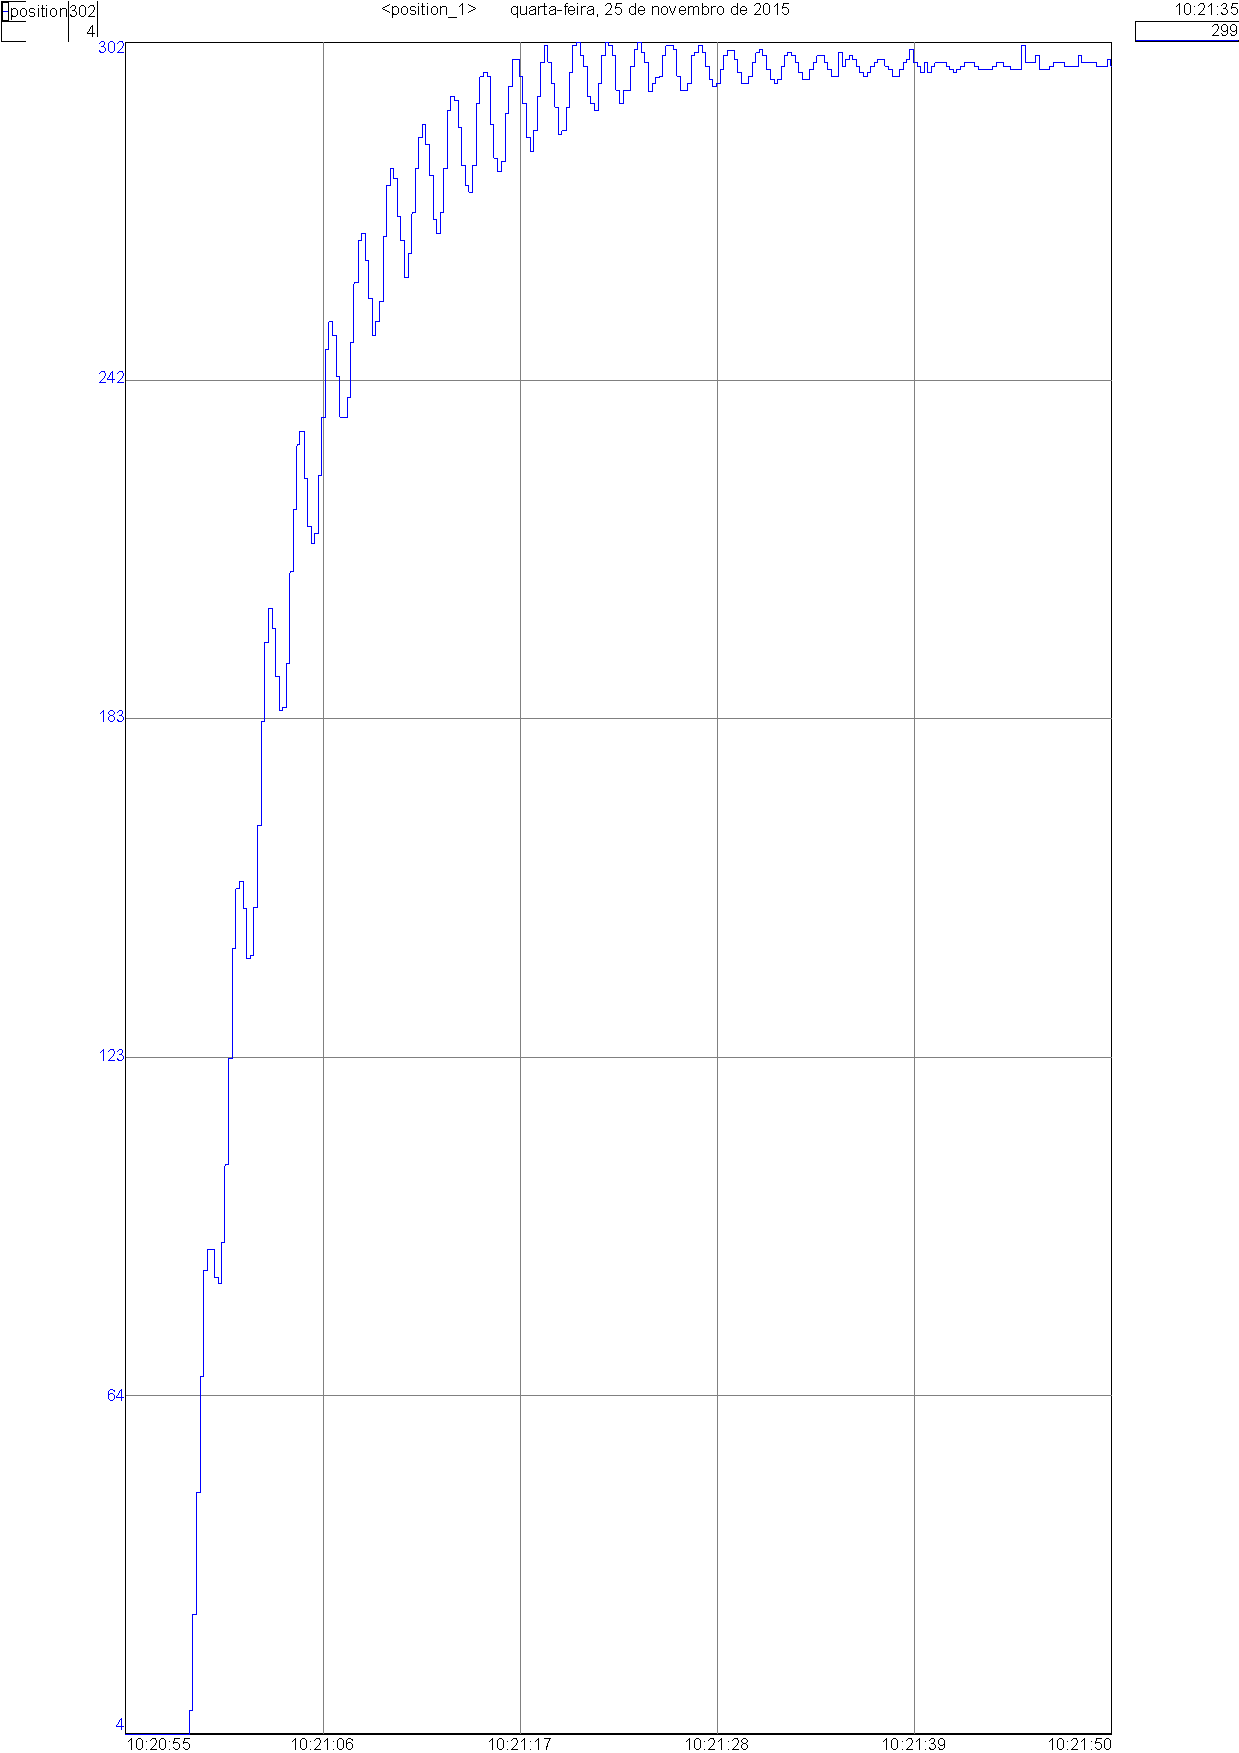
\includegraphics[width=1\linewidth,height=6cm]{figs/resultados/malha_fechada_P/MF_Proporcional_Kp_00025.pdf}
        \caption{Resultado com Malha Fechada Proporcional e $K_p = 0.0025\frac{\mathrm{u}}{\mathrm{mm}\cdot\mathrm{s}}$}
        \label{MFProporcionalKpbaixo}
    \end{minipage}%
    \hspace{0.1cm}
    \begin{minipage}{0.45\textwidth}
        \centering
        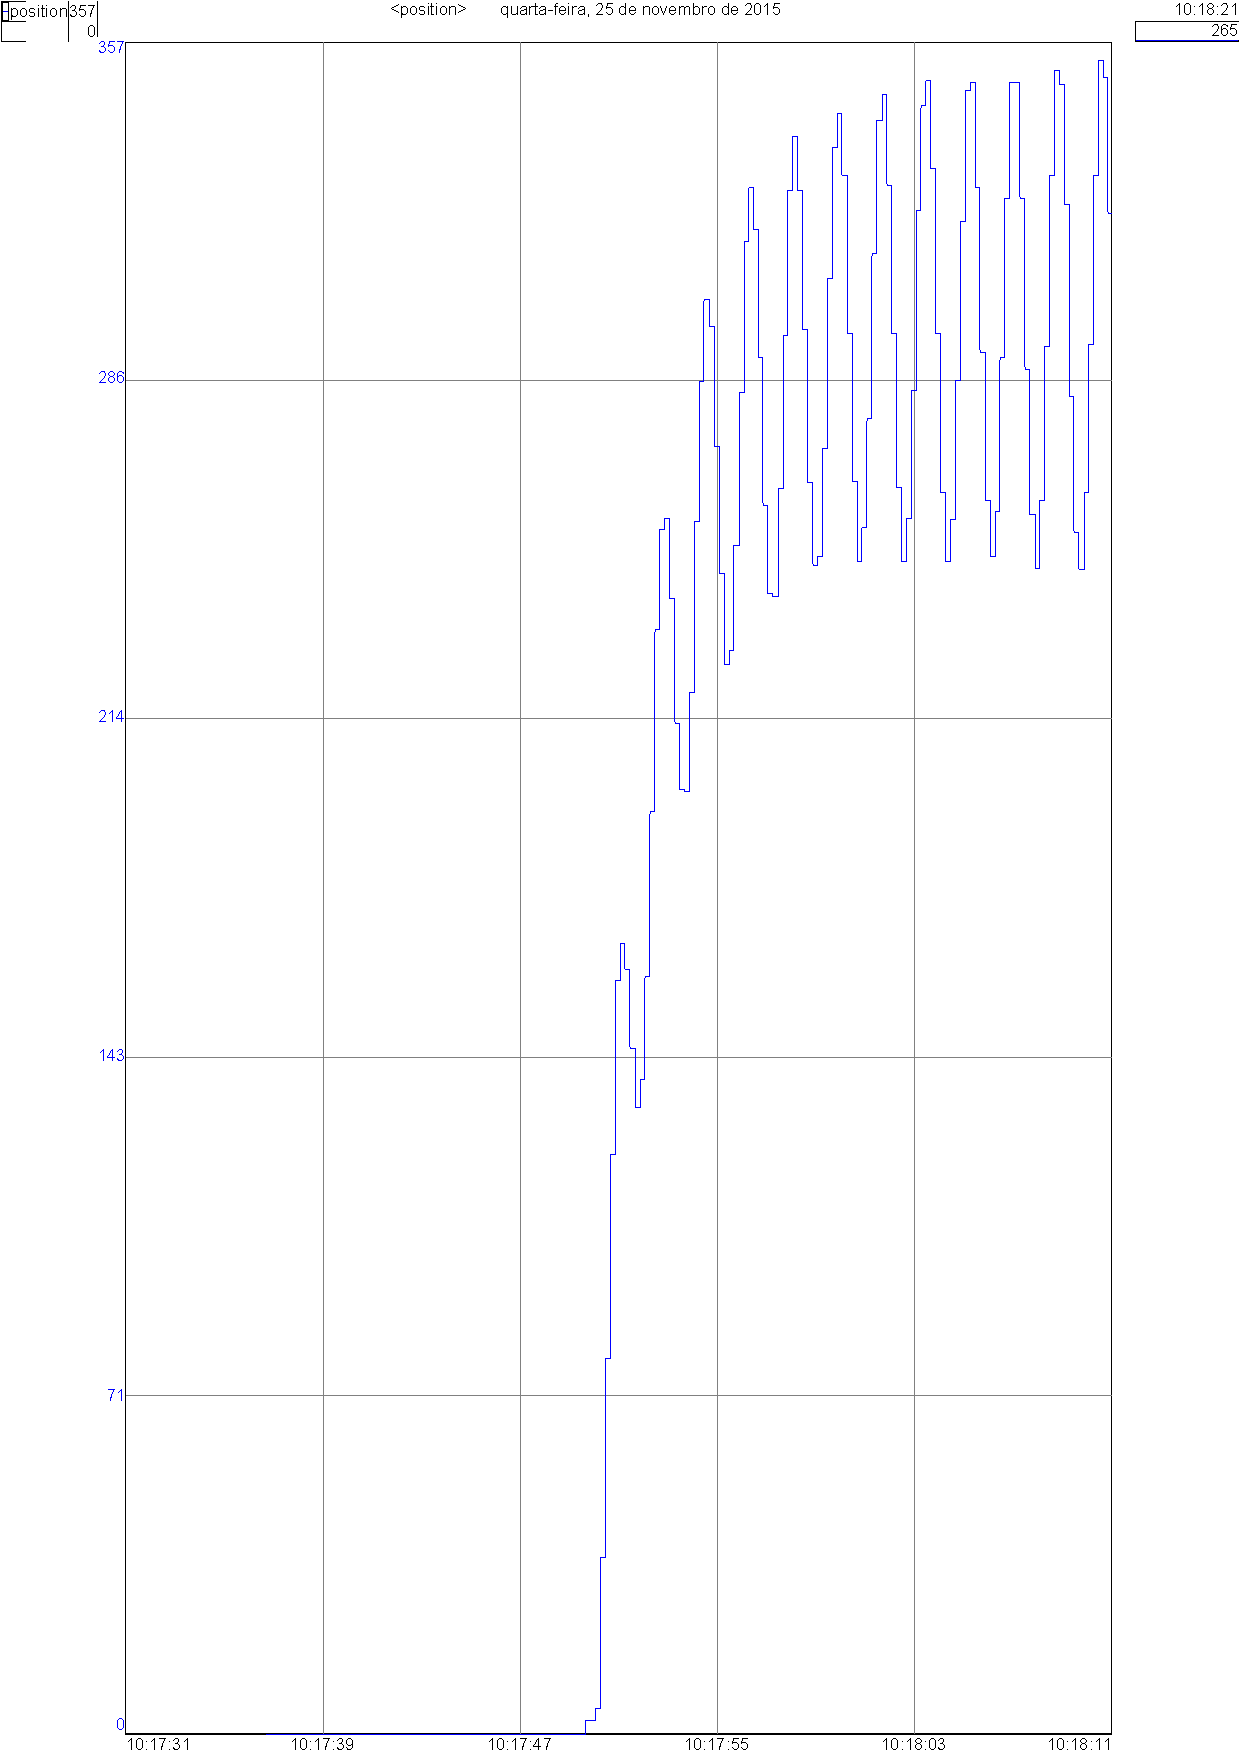
\includegraphics[width=1\linewidth,height=6cm]{figs/resultados/malha_fechada_P/MF_Proporcional_Kp_00050.pdf}
        \caption{Resultado com Malha Fechada Proporcional e $K_p = 0.0050\frac{\mathrm{u}}{\mathrm{mm}\cdot\mathrm{s}}$
        \label{MFProporcionalKpmedio}}
    \end{minipage}
\end{figure}

